\section{Introduction}
The seismic risk results are being calculated using the OpenQuake risk library (oq-risklib), an open-source suite of tools for seismic risk assessment and loss estimation. This library is written in the Python programming language and available in the form of a ``developers'' release, that can be executed through a command line interface. The code  of the library can be found on a public repository at GitHub at the following address \href{http://github.com/gem/oq-risklib}{http://github.com/gem/oq-risklib}.

This section provides a brief description of the calculators currently implemented in oq-risklib, and an initial presentation of the input and output files is provided. In the following sections, the contents and structure of these files are discussed in detail. For further information regarding the methodologies behind each calculator, users are referred to the OpenQuake-engine Book (Risk).

\section{Calculation workflows}
\label{sec:riskCalculators}
The oq-engine is currently comprised of five risk calculation workflows: two that calculate losses and damage distributions due to a single earthquake, another two that calculate seismic risk using probabilistic seismic hazard, and a fifth one that uses loss exceedance curves to assess whether retrofitting measures would be economically viable or not.

\subsection{Scenario Risk Calculator}
This calculator computes loss maps and loss statistics due to a single seismic event, for a collection of assets. The hazard input can be a single ground motion field (e.g. the median distribution of ground motion in the region of interest) or a set of ground motion fields allowing the characterisation of the inter- and intra-event variability from the GMPE. It is noted that the hazard input can either be calculated using the hazard component of OpenQuake-engine (oq-hazardlib), or provided to the risk component in an external file following the respective Natural hazards' Risk Markup Language (NRML) schema (see \href{http://github.com/gem/oq-nrmllib}{oq-nrmllib}).
A vulnerability model is combined with the distribution of the ground motions at each asset location to calculate the loss distribution for each asset, as well as the statistics of the total loss throughout the region of interest. The required input files and resulting output files are depicted in Figure \ref{fig:ScnRisk}.

\begin{figure}[ht]
\centering
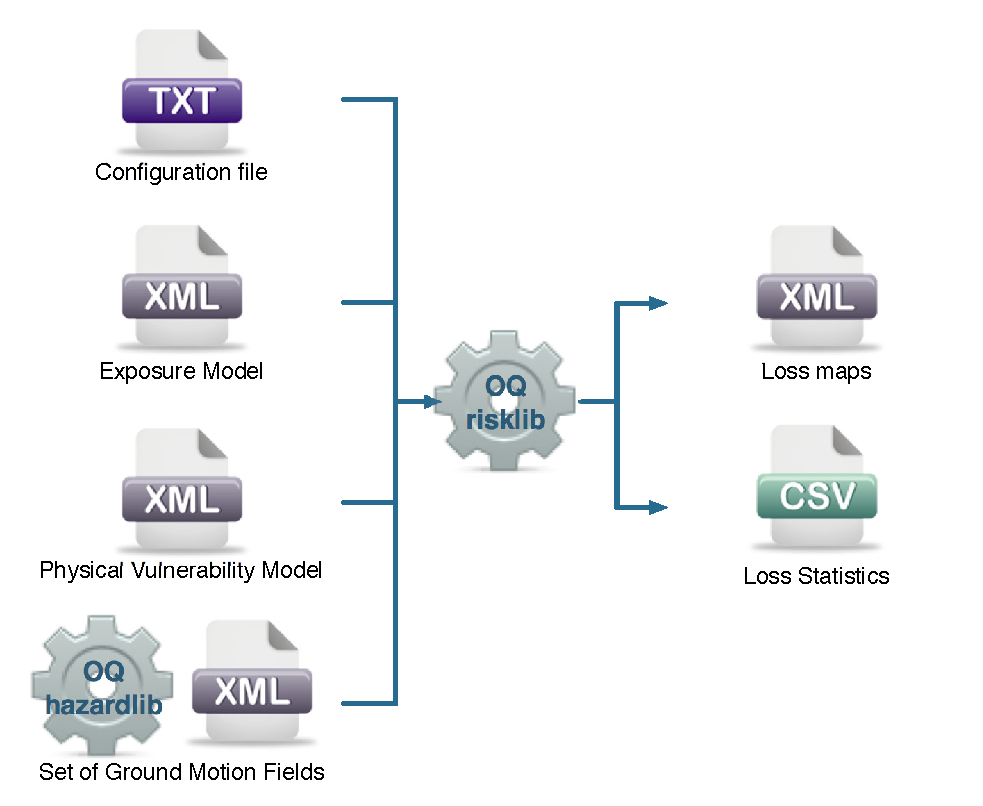
\includegraphics[width=9cm,height=7cm]{./figures/risk/ScenarioRisk.pdf}
\caption{Scenario Risk Calculator input/output structure.}
\label{fig:ScnRisk}
\end{figure}

\subsection{Scenario Damage Calculator}
This calculator is capable of assessing the damage distribution due to a single scenario earthquake, for a collection of assets. Similarly to the previous calculator, in order to perform the necessary risk calculations one or a set of ground motion fields are required, which can be derived using the oq-hazardlib, or introduced in the OpenQuake-engine using the appropriate NRML schema.
In this calculator, a fragility model is combined with the distribution of ground motion at the location of each asset, to estimate the number or area of buildings in each damage state. The damage distribution can be extracted per asset, per building typology (taxonomy) or considering all of the assets simultaneously (total damage distribution). In addition, this calculator also provides collapse maps, which contain the spatial distribution of the number or area of collapsed buildings throughout the region of interest. The input/output structure for this calculator is presented in Figure \ref{fig:ScnDamage}.

\begin{figure}[ht]
\centering
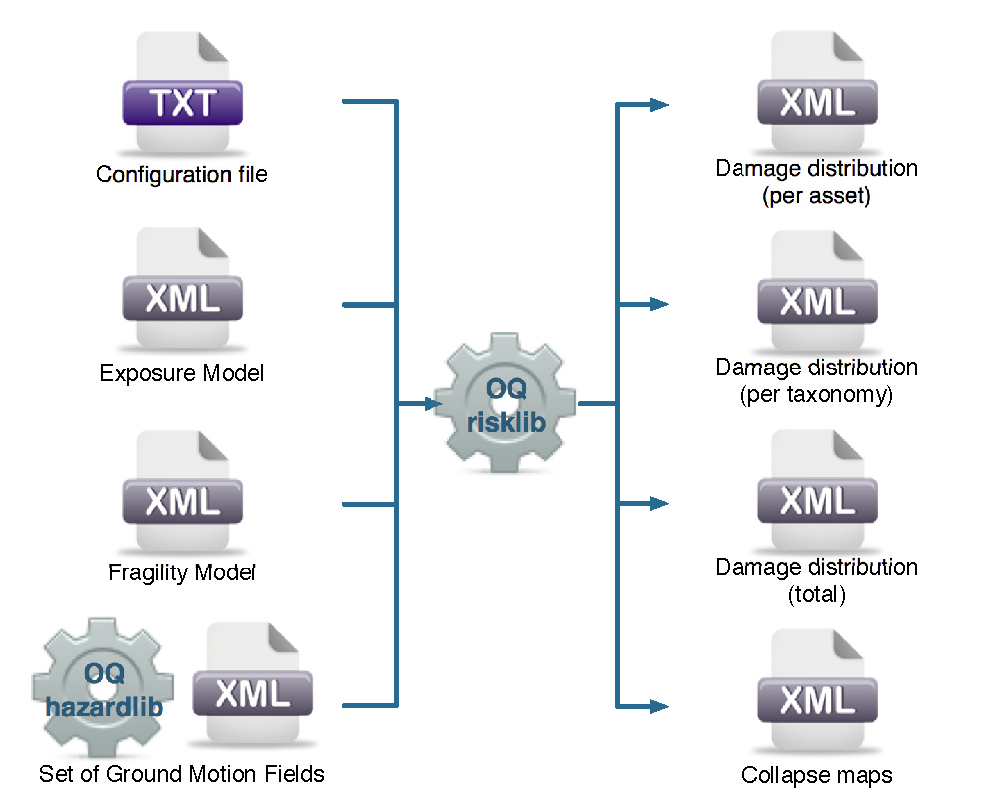
\includegraphics[width=9cm,height=7cm]{./figures/risk/ScenarioDamage.pdf}
\caption{Scenario Damage Calculator input/output structure.}
\label{fig:ScnDamage}
\end{figure}

\subsection{Probabilistic Event-based Risk Calculator}
In this calculator, loss exceedance curves and loss maps for various return periods can be calculated, based on probabilistic seismic hazard, with an event-based approach. A large number of stochastic event sets are generated, and the associated ground motion fields for each event are used together with a vulnerability model to compute the individual (per asset) and total (sum of all the losses per event) losses. Then, this distribution of losses is employed to derive a loss exceedance curve per asset, as well as a total loss exceedance curve representative of the complete building portfolio. Furthermore, oq-risklib can also compute loss maps for various return periods by interpolating each individual loss curve with the respective probability of exceedance. In Figure \ref{fig:ProbEvent}, the input/output scheme of this calculator is illustrated.

\begin{figure}[ht]
\centering
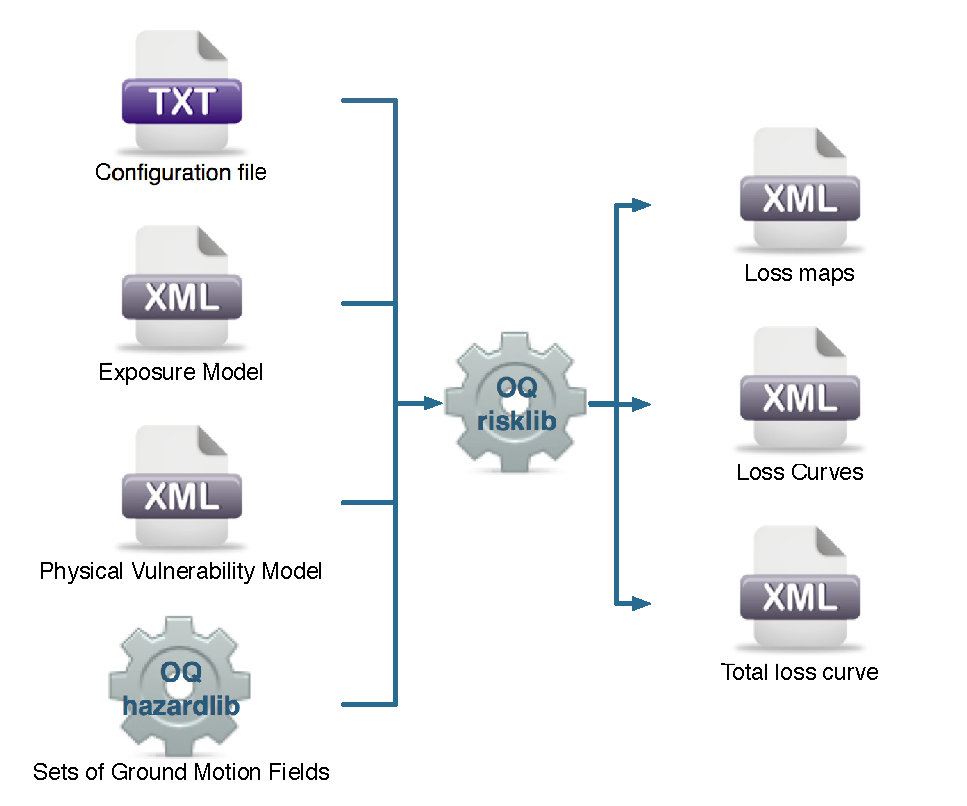
\includegraphics[width=9cm,height=7cm]{./figures/risk/ProbEvent.pdf}
\caption{Probabilistic Event-based Risk Calculator input/output structure.}
\label{fig:ProbEvent}
\end{figure}

\subsection{Classical PSHA-based Risk Calculator}
In this calculator, probabilistic seismic hazard is employed to calculate a loss exceedance curve for each asset, through the usage of seismic hazard curves. A convolution between the vulnerability function and the hazard curve at location of the asset is performed, leading to the probability of exceeding a set of loss ratios. Each loss ratio is multiplied by the asset value to obtain the final loss exceedance curve. Furthermore, probabilistic loss maps can be extracted by interpolating the loss curves at each location by various probabilities of exceedance. Unlike what was described in the previous calculator, a total loss curve (considering all assets in the exposure model) can not be extracted using this calculator, as the correlation of the ground motion residuals and vulnerability uncertainty is not taken into consideration. The input and output files involved in this calculator are presented in Figure \ref{fig:ClassicalPSHA}.

\begin{figure}[ht]
\centering
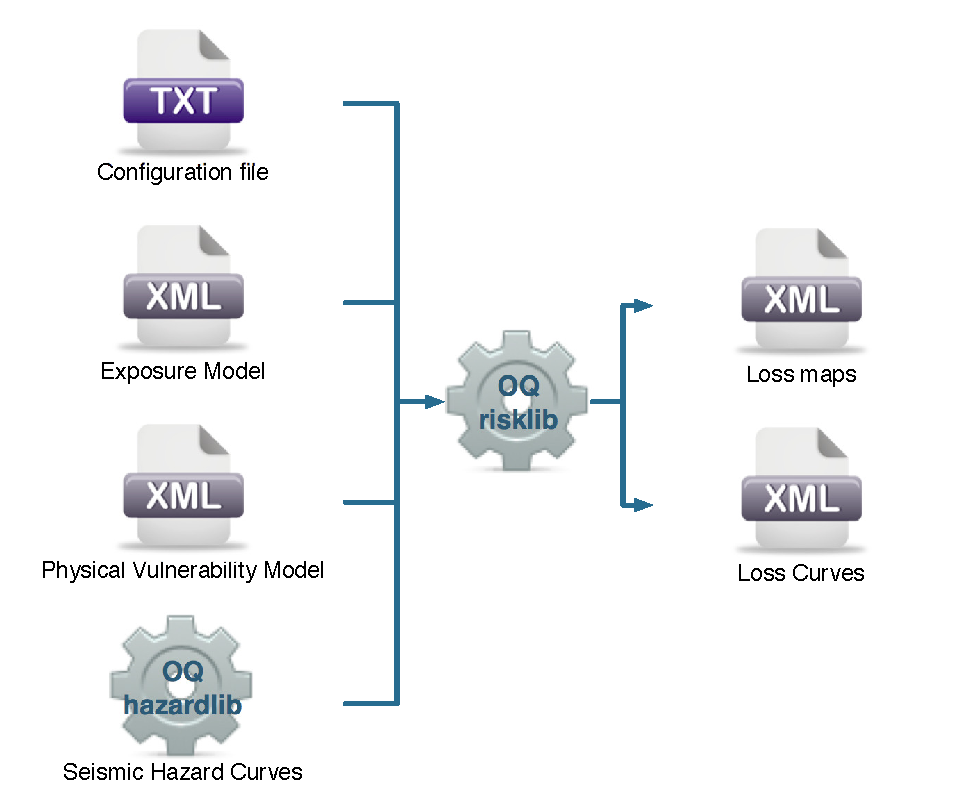
\includegraphics[width=9cm,height=7cm]{./figures/risk/ClassicalPSHA.pdf}
\caption{Classical PSHA-based Risk Calculator input/output structure.}
\label{fig:ClassicalPSHA}
\end{figure}

\subsection{Retrofitting Benefit/Cost Ratio Calculator}
This calculator represents a decision-support tool for deciding whether the employment of retrofitting measures to a collection of existing buildings is advantageous from an economical point of view. For this assessment, the expected losses considering the original and retrofitted configuration of the buildings are estimated, and the economic benefit due to the better seismic design is divided by the retrofitting cost, leading to the benefit/cost ratio. These loss curves can be computed using either the previously described Probabilistic Event-based Risk or the Classical PSHA-based Risk calculators. The output of this calculator is a benefit/cost ratio for each asset, in which a ratio above one indicates that employing  a retrofitting intervention is economically viable. In Figure \ref{fig:BCR}, the input/output structure for this calculator is depicted.

\begin{figure}[ht]
\centering
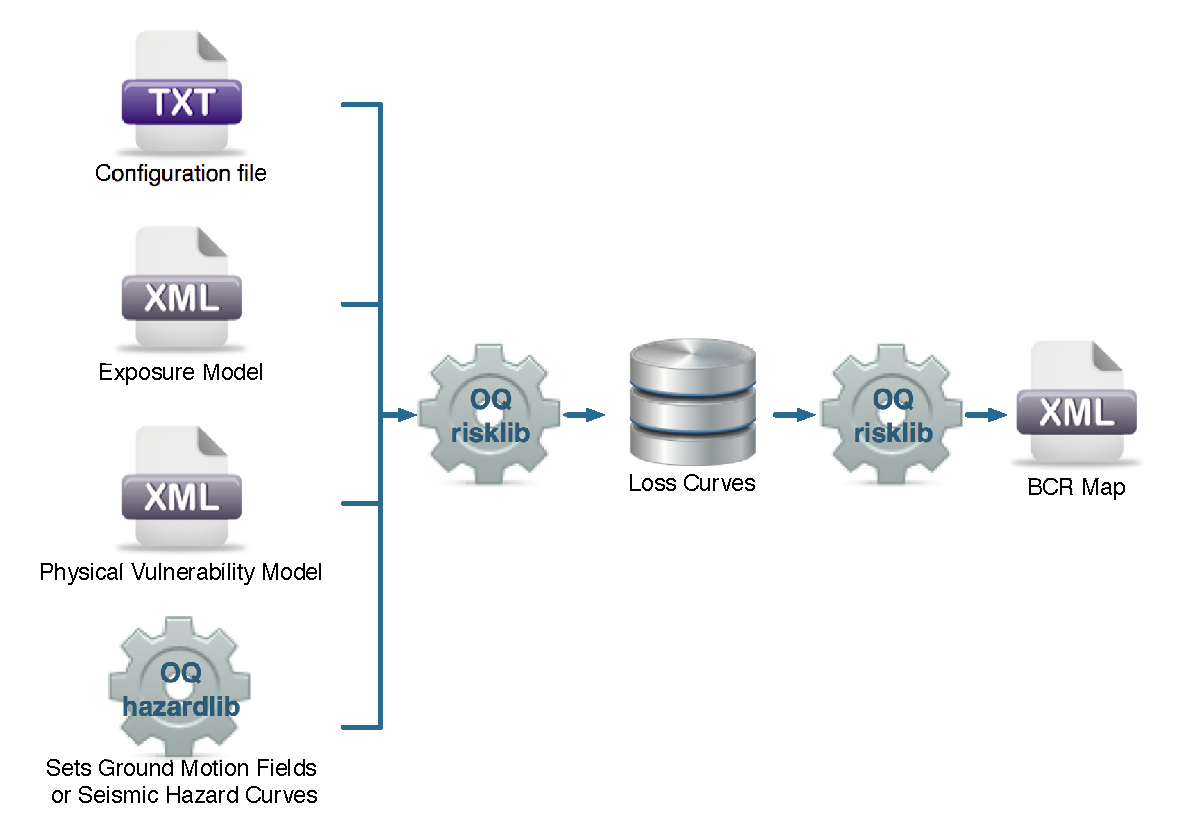
\includegraphics[width=10.5cm,height=7cm]{./figures/risk/BCR.pdf}
\caption{Retrofitting Benefit/Cost Ratio Calculator input/output structure.}
\label{fig:BCR}
\end{figure}